\documentclass[a4j,uplatex]{jsarticle}
\usepackage{amsmath}
\usepackage{amsthm}
\usepackage{amssymb}
\usepackage{amsfonts}
\usepackage{physics}
\usepackage[dvipdfmx]{graphicx}

\theoremstyle{definition}
\newtheorem{dfn}{Definition}[section]
\newtheorem*{df*}{Definition}
\newtheorem{prop}[dfn]{Proposition}
\newtheorem{lem}[dfn]{Lemma}
\newtheorem{thm}[dfn]{Theorem}
\newtheorem{cor}[dfn]{Corollary}
\newtheorem{rem}[dfn]{Remark}
\newtheorem{fact}[dfn]{Fact}
%定義の:=を書くためのやつ
\def\coloneqq{\mathrel{\mathop:}=}%
\DeclareMathOperator{\conv}{conv}

\title{数理最適化大意 課題3}
\author{理学部4年 照屋佑喜仁}

\begin{document}
\maketitle
\section{問題1}
次の線形計画問題を考える.
\begin{align*}
    \min \left\{-3x_1-2x_2:\; x\in F_\mathbb{R},\; x\in \mathbb{Z}^2\right\}
\end{align*}
ただし,$F_\mathbb{R}$は次のように定める.
\begin{align*}
    F_\mathbb{R}=\left\{(x_1,x_2)\in\mathbb{R}^2:\; x_1+3x_2\leq10,2x_1+x_2\leq4,\; x_1,x_2\geq0\right\}
\end{align*}
このとき,$F_\mathbb{R}$を図示すると以下のようになる.

\begin{figure}[h]
    \centering
    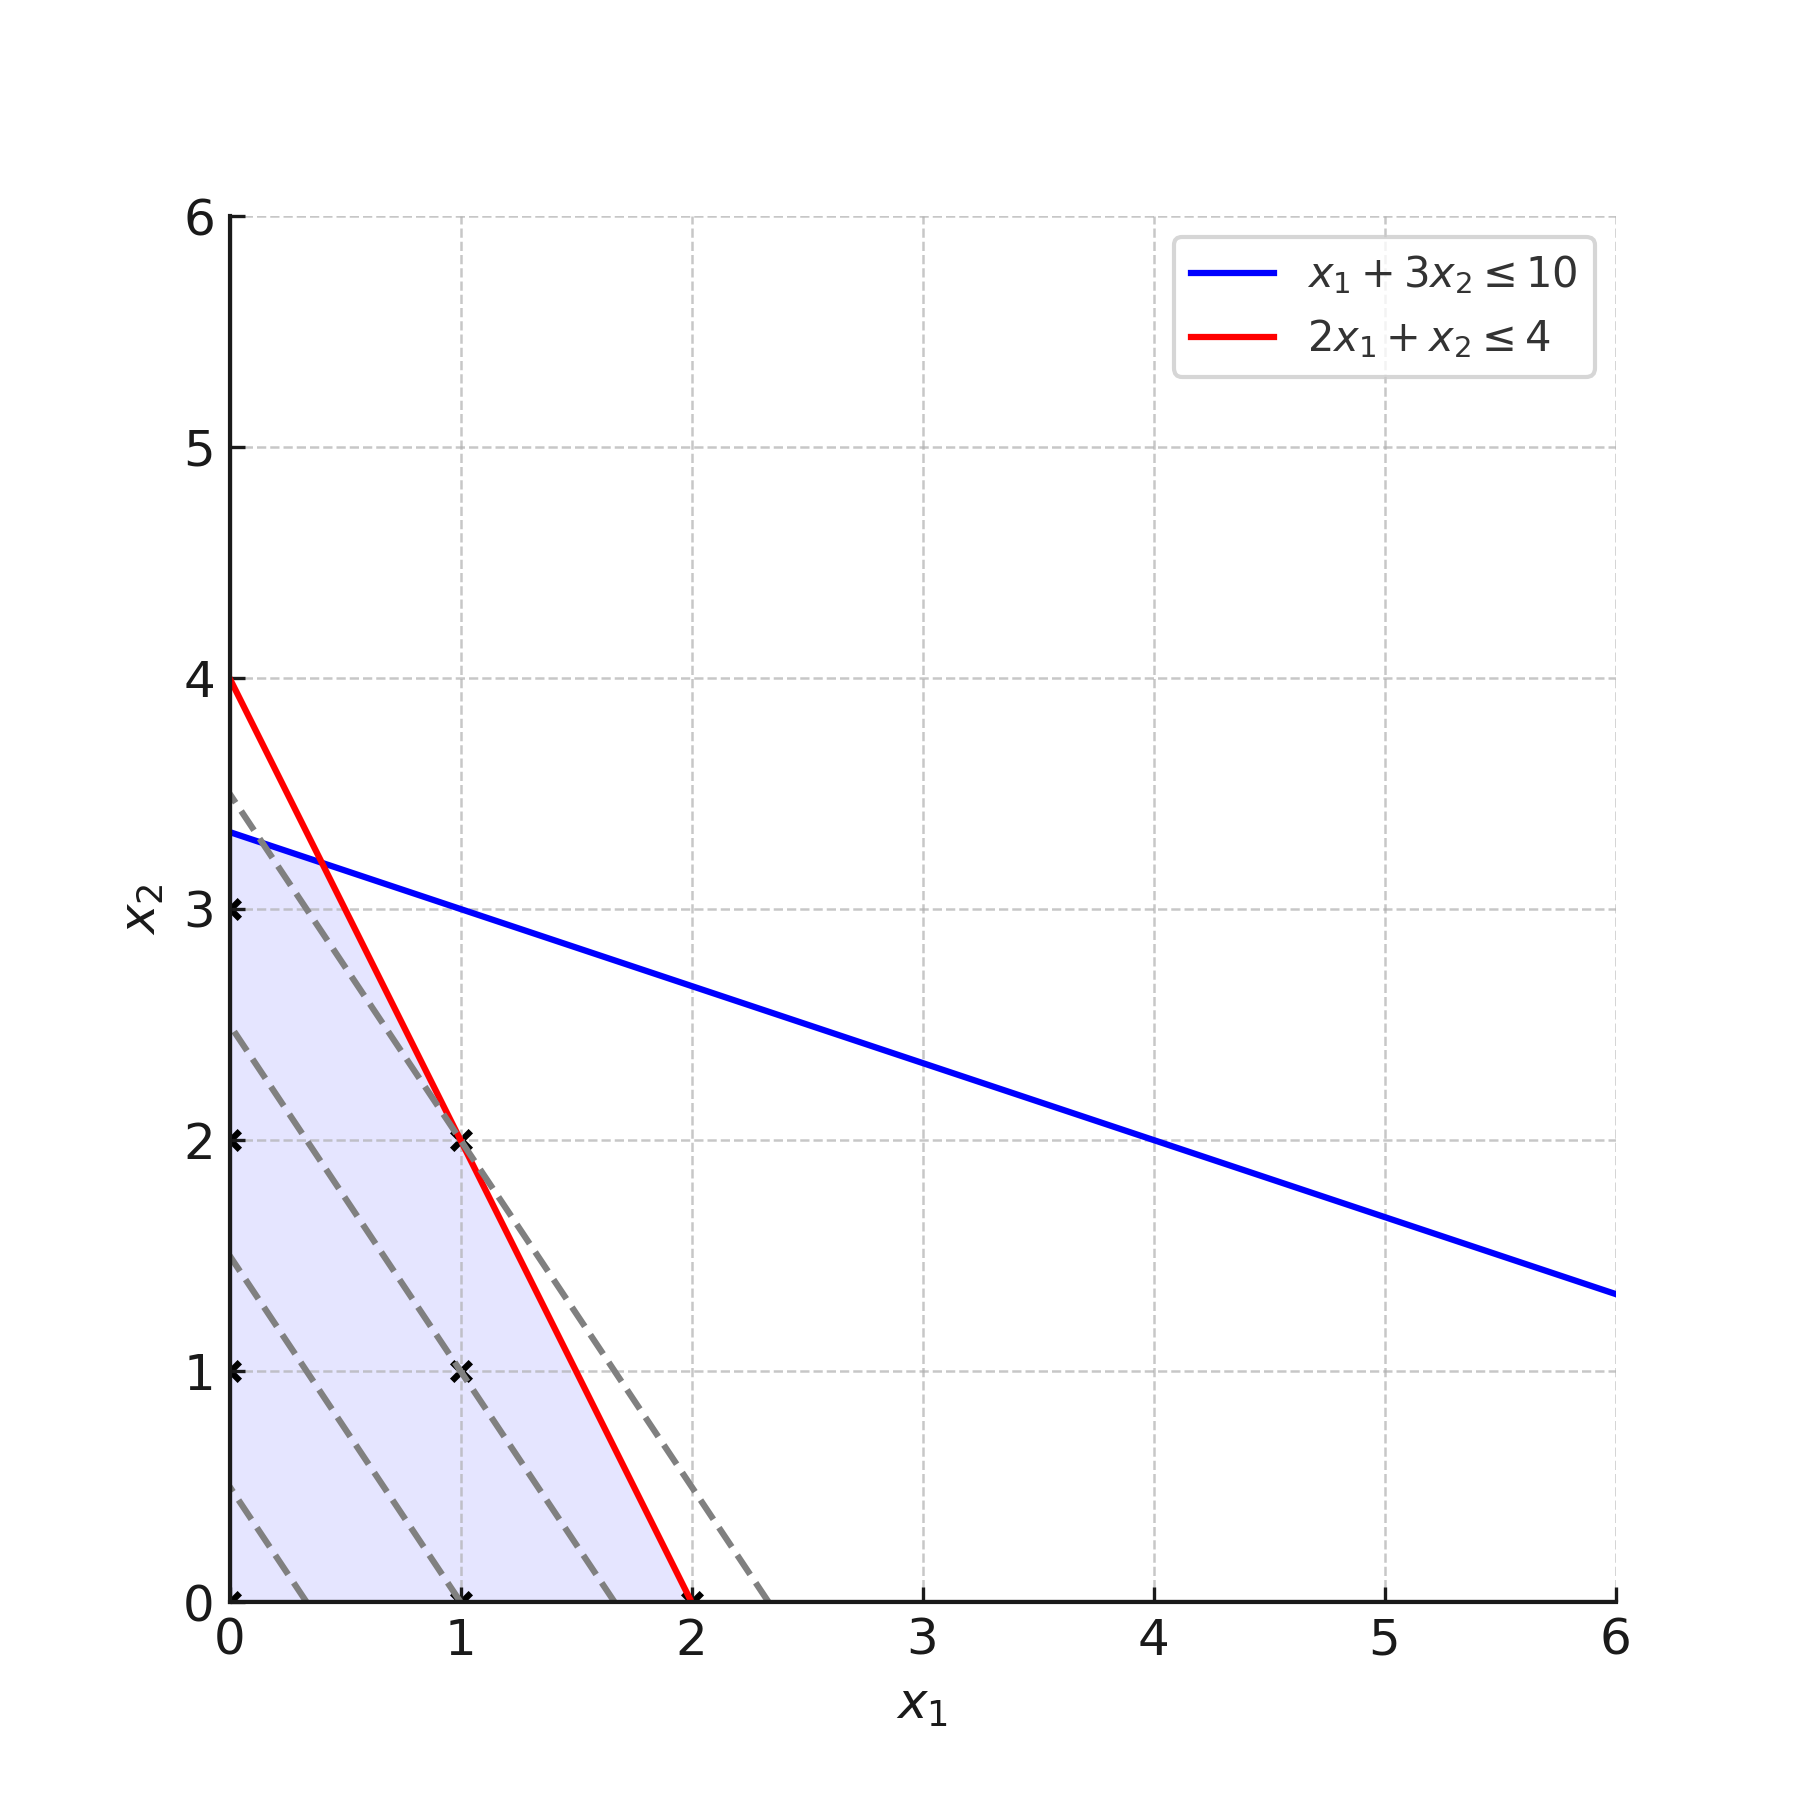
\includegraphics[width=0.6\linewidth]{lp_region_no_title.png}
    \caption{領域$F_\mathbb{R}$と$-3x_1-2x_2$の等高線}
\end{figure}
図よりこの線形計画問題の最小解は$(x_1,x_2)=(1,2)$であることがわかる.なぜなら,$-3x_1-2x_2=k$と置き$x_2$の関数と見たとき,$k$が最小になるのは直線が実行可能解の点を通ったうえで$x_2$切片が大きくなるときを考えればよいことがわかるからである.
\vskip0.5\baselineskip
次に$\conv(F_\mathbb{R}\cap\mathbb{Z}^2)$の領域を考えると以下の図を得る.

\begin{figure}[h]
    \centering
    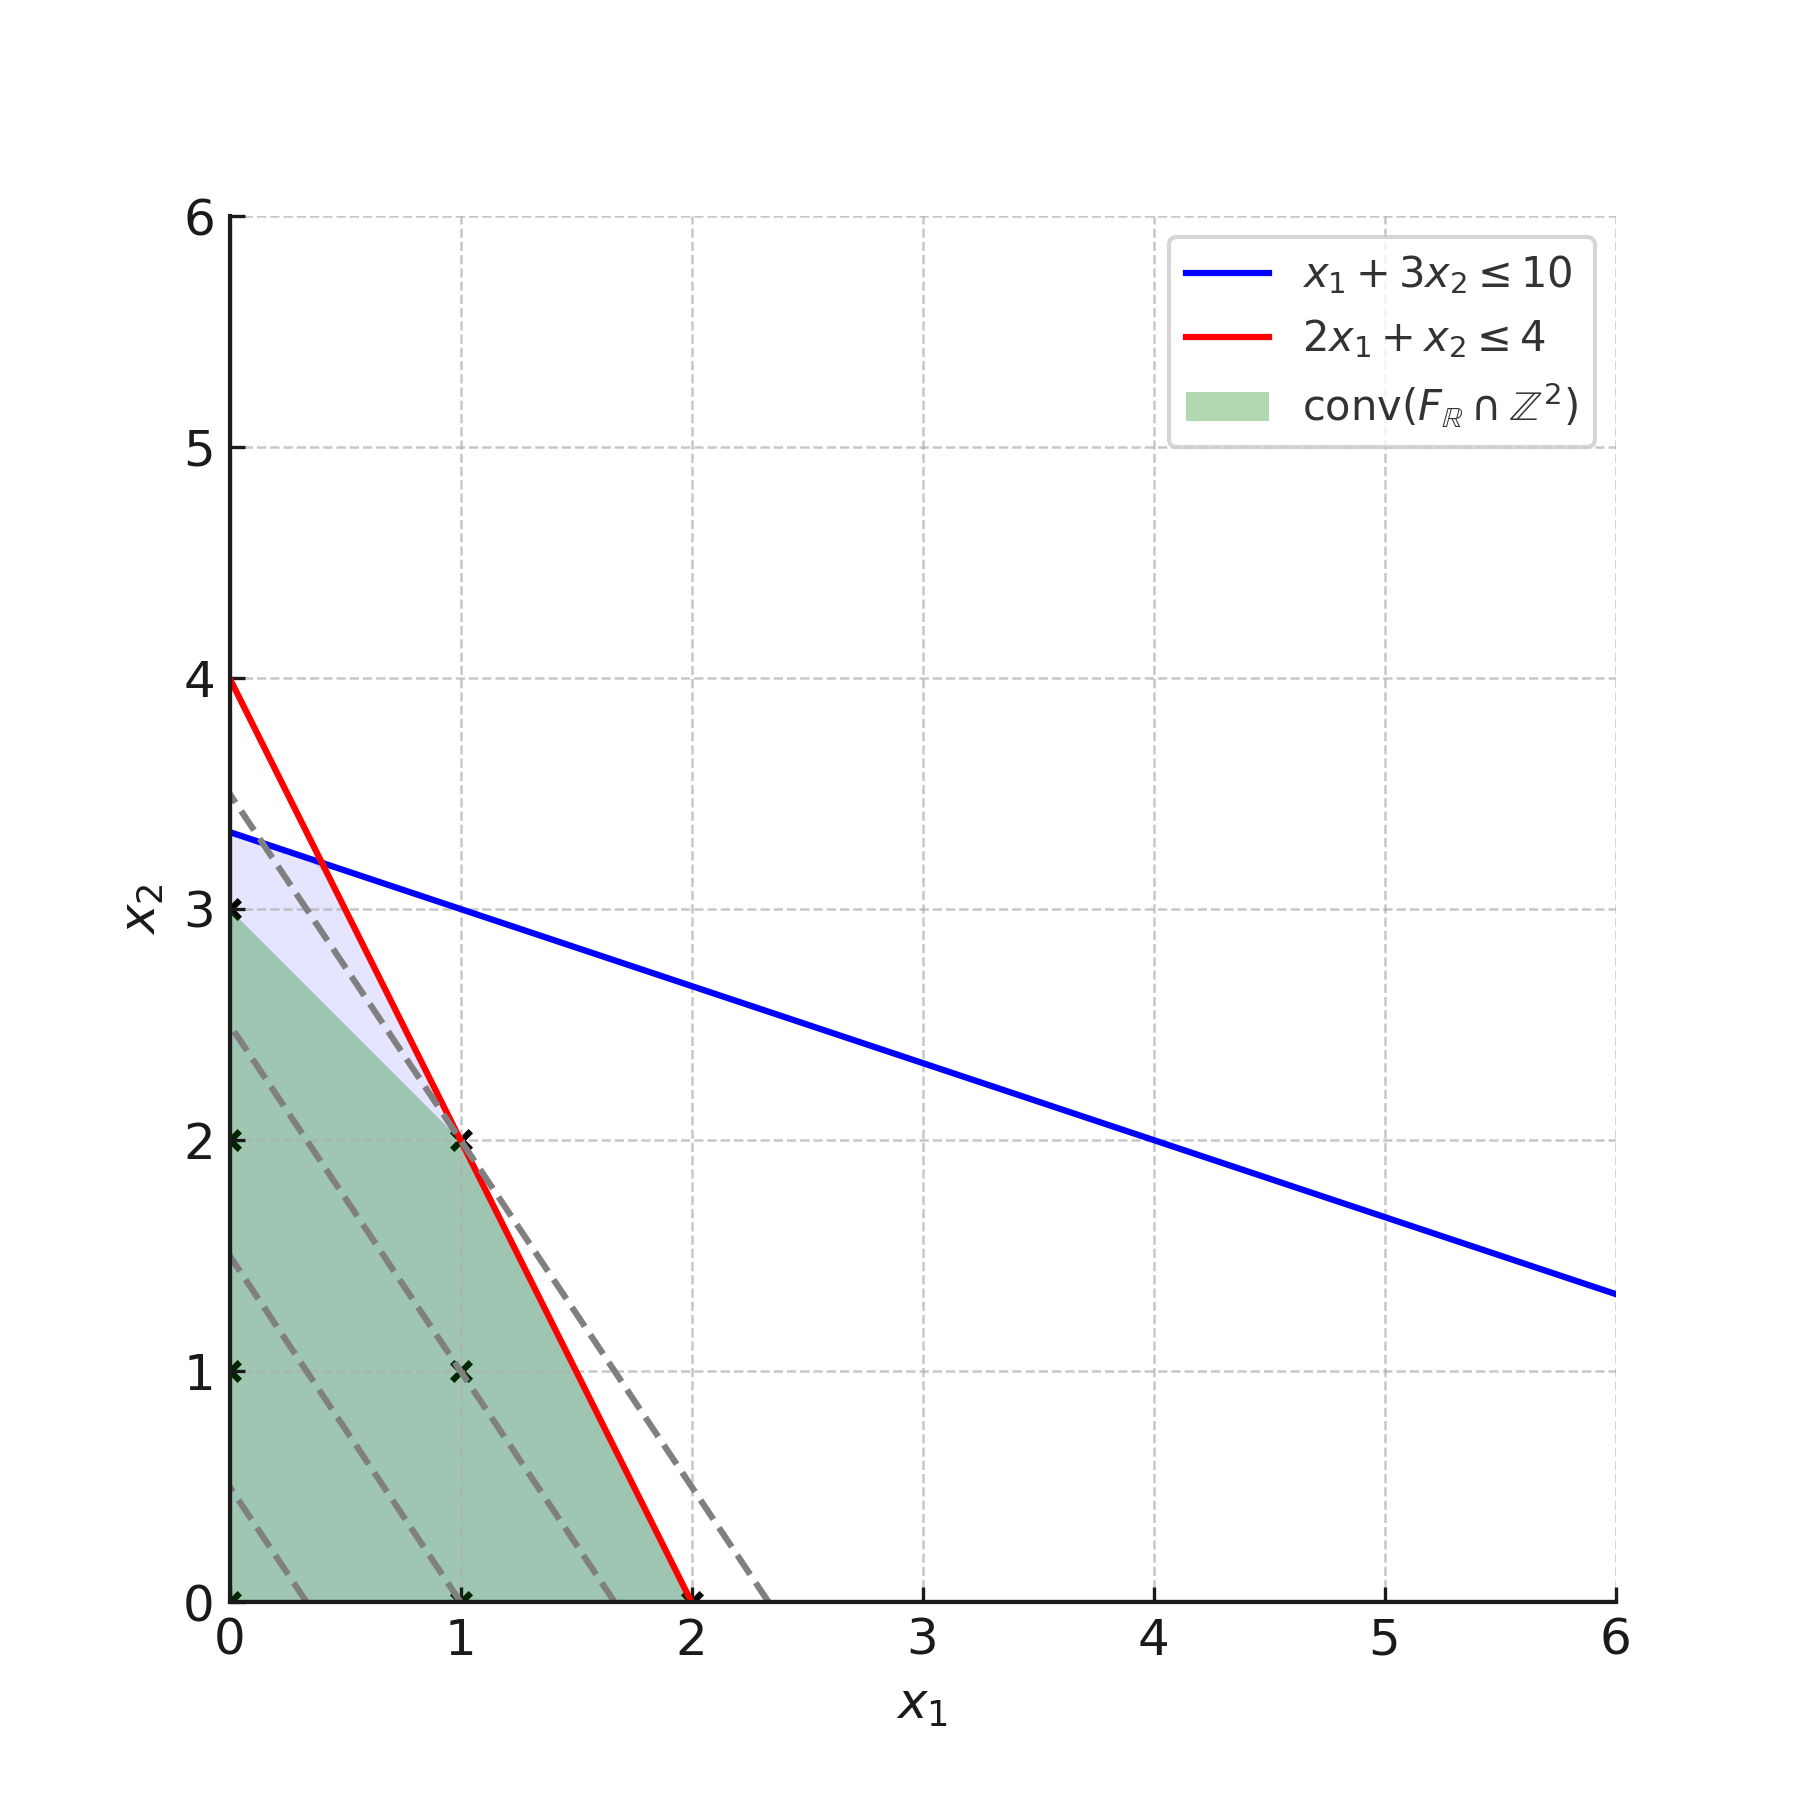
\includegraphics[width=0.6\linewidth]{lp_region_with_convex_filled.png}
    \caption{緑で囲まれた部分が$\conv(F_\mathbb{R}\cap\mathbb{Z}^2)$}
\end{figure}
図より境界は$x_2=-x_1+3,\; x_2=-2x_1+4,\; x_1=0,\; x_2=0$であることがわかるため,もとの線形計画問題と同じ最小解と最小値を持つ線形緩和問題は
\begin{align*}
    \min \left\{-3x_1-2x_2:\; x\in\tilde{F}_\mathbb{R},\; x\in\mathbb{Z}^2\right\}
\end{align*}
ただし,$\tilde{F}_\mathbb{R}$は次のように定める.
\begin{align*}
    \tilde{F}_\mathbb{R}=\left\{(x_1,x_2)\in\mathbb{R}^2:\; x_1+x_2\leq10,2x_1+x_2\leq4,\; x_1,x_2\geq0\right\}
\end{align*}

\end{document}
